\chapter{ARTICULAÇÃO COM OS VALORES, PRINCÍPIOS E POLÍTICAS DE ENSINO DA UTFPR}

Este Capítulo é uma complementação do \autoref{chap:politicas}, apresentado a estruturação das políticas de ensino da UTFPR no âmbito do Curso de Engenharia Eletrônica, tendo como base a matriz curricular apresentada no \autoref{chap:matriz}.

\section{DESENVOLVIMENTO DA ARTICULAÇÃO ENTRE A TEORIA E A PRÁTICA}

O curso de Engenharia Eletrônica define quatro instrumentos para desenvolver a articulação entre a teoria e a prática: (i) atividades práticas em unidades curriculares, (ii) projetos práticos interdisciplinares, (iii) estágio curricular obrigatório e (iv) Trabalho de Conclusão de Curso (TCC).

Neste sentido, a matriz curricular do curso de Engenharia Eletrônica apresenta 34 (trita e quatro) unidades curriculares que contemplam carga horária prática, totalizando \the\value{horasAP} horas de atividades práticas. Informações mais detalhadas sobre esta distribuição podem ser observadas no \autoref{qua:matriz} na \autoref{sec:matriz}, Matriz Curricular.

Além disso, os docentes são encorajados a aplicarem projetos práticos interdisciplinares, onde experiências práticas de implementação de projetos são propostas aos discentes, complementando a articulação entre teoria e prática, e inserindo a perspectiva de interdisciplinaridade no curso. Tipicamente, tais projetos são desenvolvidos nas unidades curriculares de Sistemas Digitais, Microcontroladores, Sistemas Embarcados, Medidas e Sensores e Eletrônica de Potência.

O estágio curricular obrigatório contabiliza 400 h de atividades, podendo ser iniciado a partir do 7\textordmasculine{} período. Neste contexto, o estudante é capaz de colocar em prática todo o ensinamento recebido durante seus anos de estudo no curso, sendo acompanhado por um professor orientador e um supervisor responsável pelo estágio na empresa que o oferece. Para possibilitar um melhor aproveitamento do discente em relação ao Estágio, este PPC foi desenvolvido prevendo a redução de carga horária no nono e décimo período. Desta forma, o discente tem condições de buscar oportunidades de estágio em outras regiões, dentro e fora do país.

Assim como o estágio obrigatório, o TCC é capaz de colocar em prática todo o ensinamento recebido pelo discente durante o curso, sendo acompanhado por um(a) docente orientador(a). Os(as) orientadores, em consonância com a atuação do docente responsável pelas atividades de TCC, buscam sempre a realização de projetos práticos e interdisciplinares, como é caso do desenvolvimento de processos, produtos ou protótipos.

\section{DESENVOLVIMENTO DAS COMPETÊNCIAS PROFISSIONAIS}
\label{sec:comp}

Assim como citado na \autoref{sec:perf}, neste PPC são propostas seis Competências Específicas para o egresso do curso: Básica, Computação, Eletrônica, Científica, Empreendedora e Eletrotécnica. As competências são desenvolvidas gradativamente em várias unidades curriculares e em momentos distintos no decorrer do curso. Em alguns casos, unidades curriculares são comuns a mais de uma competência.

\subsection{A competência Básica}

Ao conquistar essa competência, o discente será capaz de \textbf{resolver problemas estruturados de diferentes contextos das Engenharias, de maneira autorregulada, integrando conhecimentos das áreas de química, física e matemática, utilizando raciocínio lógico quantitativo e ferramentas tecnológicas}. As Unidades Curriculares necessárias para esta competência são: Introdução à Engenharia, Cálculo Diferencial e Integral 1, 2, 3 e 4B; Cálculo numérico; Probabilidade e estatística; Física 1, 2, 3 e 4; Química Básica Teórica e Experimental; Mecânica 1; Fenômenos de Transporte e Eletromagnetismo.

\subsection{A competência de Computação}

Ao conquistar essa competência, o discente será capaz de \textbf{conceber e/ou intervir em sistemas computacionais com autonomia nos diferentes contextos da engenharia, de maneira organizada e lógica, integrando a eletrônica analógica e digital, considerando uma documentação clara e concisa}. As Unidades Curriculares necessárias para esta competência são: Computação 1, Fundamentos de Programação, Arquitetura e Organização de Computadores, Cálculo numérico e Sistemas operacionais.

\subsection{A competência de Eletrônica}

Ao conquistar essa competência, o discente será capaz de \textbf{conceber e/ou intervir em sistemas eletrônicos com autonomia, integrando circuitos analógicos, computação embarcada, controle de sistemas e processamento digital de informações e considerando uma documentação clara e concisa}. Para conquistar a competência de Eletrônica é necessário que o discente seja aprovado em quatro ramos de unidades curriculares que compreendem quatro áreas de atuação, sendo elas:

\begin{itemize}
    \item Eletrônica Analógica;
    \item Sistemas Embarcados;
    \item Processamento Digital de Sinais; e
    \item Sistemas de Controle.
\end{itemize}

As Unidades curriculares necessárias para cada área estão dispostas na \autoref{fig:copele}. Pode-se notar que em cada ramo da Competência de Eletrônica existem unidades curriculares destacadas (sublinhadas), sendo responsáveis por integrar o conhecimento de cada área área de atuação.

\begin{figure}[!htb]
    \centering
    \caption[Áreas e unidades curriculares da Competência de Eletrônica]{Áreas e unidades curriculares da Competência de Eletrônica}
    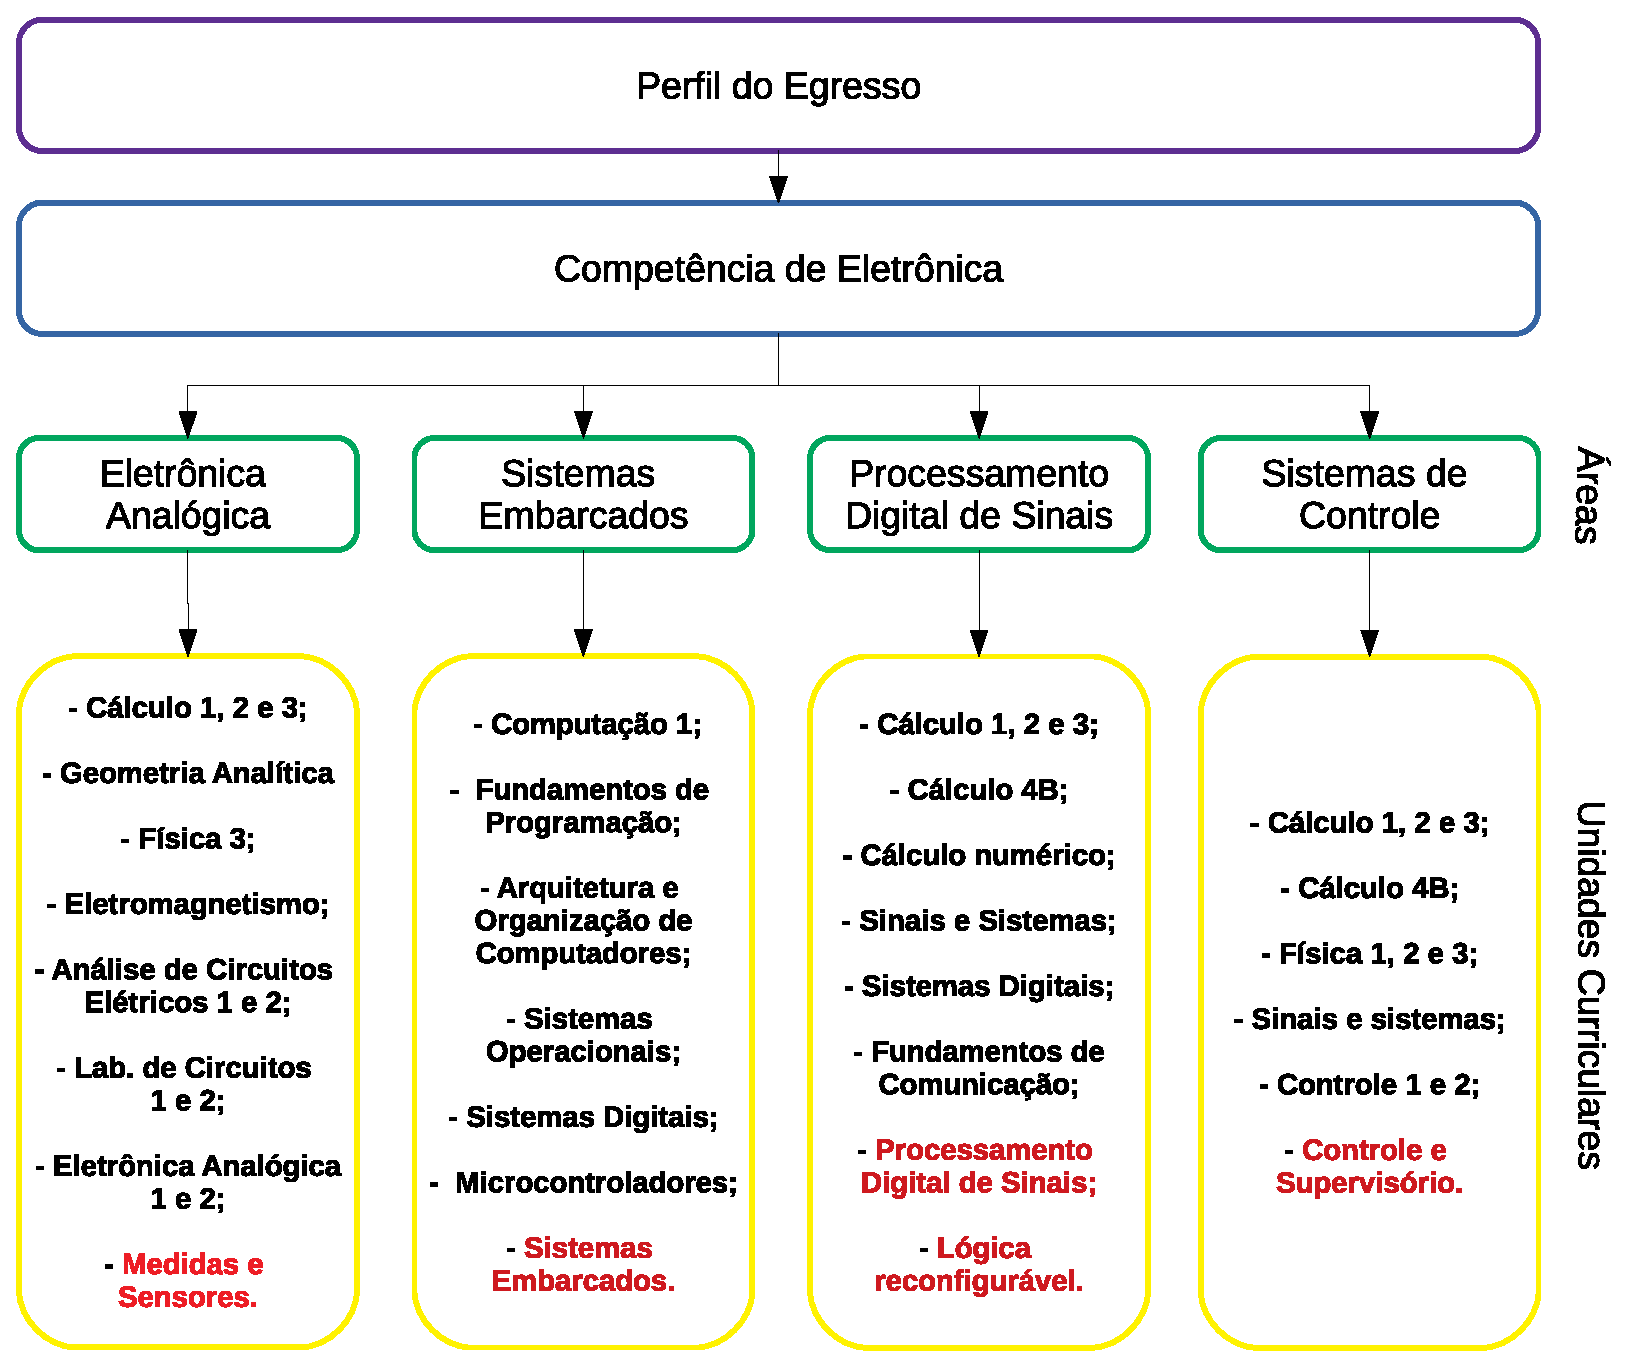
\includegraphics[width=1.0\textwidth]{Caps/Figs/comp_eletronica.eps}
    \fonte{\utf}
    \label{fig:copele}
\end{figure}

\subsection{A competência de Científica}

Ao conquistar essa competência, o discente será capaz de \textbf{produzir investigação científica integrando modelos de fenômenos naturais, conhecimentos técnico-científicos, escrita e metodologia científica com honestidade intelectual e senso crítico}. As unidades curriculares necessárias para esta competência são Metodologia da Pesquisa, Trabalho de Conclusão de Curso 1 e Trabalho de Conclusão de Curso 2. Cabe destacar que para a estruturação dessa competência cada discente precisa aplicar os conhecimentos e as demais competências adquiridas no decorrer do curso.

\subsection{A competência Empreendedora}

Ao conquistar essa competência, o discente será capaz de \textbf{analisar ou propor negócios, com responsabilidade compartilhada e atitudes empreendedora e cooperativa, por meio da articulação de informações técnicas e conceituais e avaliação do micro e macroambiente}. Para a extruturação da competência, o discente precisa cursar algumas unidades curriculares optativas do ciclo de humanidades: Gestão de Projetos, Empreendedorismo, Ciências do Ambiente e uma unidade curricular da área de Economia.

\subsection{A competência de Eletrotécnica}

Ao conquistar essa competência, o discente será capaz de \textbf{conceber e/ou intervir em sistemas elétricos com autonomia, integrando instalações elétricas , máquinas elétricas e sistemas de potência, considerando uma documentação clara e concisa e segurança elétrica}. As unidades curriculares necessárias para esta competência são: Análise de Circuitos Elétricos 1 e 2; Laboratório de Circuitos Elétricos 1 e 2; Materiais e Equipamentos Elétricos; Eletromagnetismo; Fundamentos de Engenharia de Segurança no Trabalho; Conversão de Energia 1; Máquinas e Acionamentos; Instalações Elétricas; Instalações Industriais; Geração, Transmissão e Distribuição de Energia Elétrica e Sistemas de Potência.

É importante ressaltar que as unidades curriculares de Instalações Industriais; Geração, Transmissão e Distribuição de Energia Elétrica e Sistemas de Potência são optativas. Dessa forma, o discente precisa cursá-las para adquirir a competência. Ademais, o egresso que cursar essas disciplinas atenderá a carga horária mínima para a obtenção da atribuição de Engenheiro Eletricista pelo CREA (Artigo 8\textordmasculine{} da Resolução CONFEA 218/1973 \cite{confea1973}).

\section{DESENVOLVIMENTO DA FLEXIBILIDADE CURRICULAR}

Assim como discutido na \autoref{sec:flex}, o curso apresenta duas modalidades de flexibilização curricular: \textbf{vertical} e \textbf{horizontal}. 

A flexibilização vertical é realizada pela organização das unidades curriculares ao longo dos semestres compreendendo o núcleo de formação específica do curso. Dessa forma, os turnos das Unidades Curriculares são alocados preferencialmente de forma alternada entre manhã e tarde na sequencia dos semestres. Isso permite que os discentes possam adiantar conteúdos do próximo semestre. Também possibilita que alguém que não obteve a aprovação em uma unidade curricular, possa cursá-la sem necessidade de deixar de cursar os conteúdos do semestre em que se encontra.

Além disso, existem dois momentos onde os discentes possuem liberdade para orientar seu caminho acadêmico, o primeiro momento ocorre a partir do 3\textordmasculine{} período por meio da escolha de cinco ``Optativas do Colégio de Humanidades''. Em um segundo momento, a partir do 7\textordmasculine{}, os discentes podem escolher três optativas das áreas de aprofundamento.

\section{DESENVOLVIMENTO DA MOBILIDADE ACADÊMICA}

\section{DESENVOLVIMENTO DA INTERNACIONALIZAÇÃO}

\section{DESENVOLVIMENTO DA ARTICULAÇÃO COM A PESQUISA E PÓS GRADUAÇÃO}

\section{DESENVOLVIMENTO DA EXTENSÃO}

\subsection{Projetos e unidades curriculares extensionistas}